\documentclass[11pt,a4paper]{article}
\usepackage[utf8]{inputenc}
\usepackage[T1]{fontenc}
\usepackage{amsmath,amsfonts,amssymb}
\usepackage{apacite}
\usepackage{natbib}
\usepackage{graphicx}
\usepackage{booktabs}
\usepackage{threeparttable}
\usepackage{array}
\usepackage{url}
\usepackage{hyperref}
\usepackage[margin=2.5cm]{geometry}
\usepackage{setspace}
\usepackage{comment}
\usepackage{outlines}
\onehalfspacing

\newcommand{\Var}{\text{Var}}
\newcommand{\Cov}{\text{Cov}}

% Define \sym command for significance stars from esttab
\newcommand{\sym}[1]{{#1}}

\title{CEO Replacements and Firm Growth: Correcting for Small-Sample Bias in Fixed-Effect Estimates\thanks{We thank Otavio Bartalotti and St\'ephane Bonhomme for helpful discussions and comments and the seminar participants at the Universit\'a della Svizzera Italiana and Corvinus Empirical Seminar for comments. Project no. 144193 has been implemented with the support provided by the Ministry of Culture and Innovation of Hungary from the National Research, Development and Innovation Fund, financed under the KKP\_22 funding scheme. This project was funded by the European Research Council (ERC Advanced Grant agreement number 101097789). Telegdy received support from the Hungarian Scientific Research Fund – OTKA, contract number 143346. The views expressed in this research are those of the authors and do not necessarily reflect the official view of the European Union or the European Research Council.}}

\author{Miklós Koren\thanks{Central European University, ELTE Centre for Economic and Regional Studies, CEPR and CESifo. E-mail: korenm@ceu.edu} \\
        Krisztina Orbán\thanks{Monash University. E-mail: krisztina.orban@monash.edu} \\
        Álmos Telegdy\thanks{Corvinus University of Budapest. E-mail: almos.telegdy@uni-corvinus.hu}}

\date{October 2025}

\begin{document}

\maketitle
\thispagestyle{empty}

\begin{abstract}
\noindent
We study how much CEO replacements contribute to firm growth and show that traditional fixed effect estimates substantially overstate CEO influence and create spurious trends due to small-sample bias. We introduce a placebo-controlled, difference-in-differences method using non-changing firms to correct bias in second moments. Simulations confirm the method is robust to persistent shocks, short tenures, and unbalanced panels. Naive estimates on 60,000 Hungarian CEO transitions attribute 40–60\% of revenue variance to CEO changes, our debiased method finds 20-30\%. The corrected estimates show immediate, persistent effects without false pre-trends.
\end{abstract}

\textbf{Keywords:} CEO value, CEO-Firm Fixed Effects, Bias Correction

\textbf{JEL Classification:} C23, D24, G34

\clearpage
\setcounter{page}{1}

%%%%%%%%%%%%%%%%%%%%%%
\section{Introduction}
%%%%%%%%%%%%%%%%%%%%%%

The impact of individual CEOs on business practices and firm performance is a widely studied question in economics, corporate finance, and management. In the absence of direct measures of CEO characteristics relevant for firm outcomes, studies often include CEO fixed effects to capture variations in latent CEO skills \citep{Bertrand2003-io, crossland2011differences, quigley2015has}. 

Most applied work uses second moments of the estimated fixed effects to understand the importance of CEOs in shaping firm behavior. Variance decompositions reveal how much CEOs contribute to the variance of firm outcomes. Firm attributes, such as profitability \citep{mackey2008effect} and risk \citep{schoar2024effect}, are often regressed on the estimated CEO effect, where the estimated coefficient contains the covariance between the dependent variable and the fixed effect. Finally, event studies are used to assess how outcomes evolve before and after CEO transitions to test for pre-trends and to understand post-transition dynamics \citep{schoar2024effect}. However, both the variance and the covariance of estimated fixed effects are biased upwards by small-sample noise even under credible identification assumptions
\citep{andrews2008high,gaure2014correlation,bonhomme2023much}, which leads to biased second moments and distorts inferences about CEO effects. The bias arises because fixed effect estimates are only T-consistent and not N-consistent: adding more firms does not eliminate noise in individual CEO estimates when each CEO has short tenure at few firms. The bias also introduces spurious pre-trends and distorts post-transition dynamics in event studies when errors are autocorrelated.\footnote{To date, we did not find any study addressing the issue of spurious pre-trends.} This spurious pre-trend problem is particularly concerning for applied researchers, who use pre-trend tests to validate identification strategies. When mechanical bias generates pre-trends, researchers may mistakenly reject valid designs.

The literature offers a number of approaches to correct for the bias in the variance and covariance of estimated fixed effects. We are not aware of other methods that correct the dynamic bias, which we show to be prevalent in event study designs. In terms of variance-covariance correction, three broad methods are proposed: assuming and estimating a parametric model for error covariance structure \citep{andrews2008high,gaure2014correlation,kline2024firm}, leave-one-out adjustments \citep{kline2020leave}, and grouping observations to reduce the number of parameters to be estimated \citep{Bonhomme2019-xi,bonhomme2023much}. Parametric methods require correctly specifying and estimating complex autocorrelation patterns, while the leave-one-out method is impractical in CEO markets where most managers work at only one firm and mobility is limited. Since our interest is understanding heterogeneity of CEOs and factors that correlate with this heterogeneity, keeping the original dimensionality of the data is preferable. 

We propose a placebo-controlled correction method. We match CEO-changing firms with non-changing firms from the same sector and cohort, then assign fake CEO transitions at the same calendar year to the control firms.\footnote{Using firms which do not change CEO to control for noise in the data is in the spirit of \cite{fitza2014use} and \cite{jarosiewicz2023revisiting}.} Because placebo firms do not change CEOs, any variance or covariance in their estimated CEO effects is pure bias. Under reasonable assumptions, the placebo group measures the exact bias in variance, covariance, and event-study dynamics. Differencing treated and placebo second moments yields debiased estimates without modeling the full error structure. This approach sidesteps both the parametric modeling requirements and the limited-mobility problem that plague existing methods of variance correction allows for debiased event study coefficients.\footnote{Because CEOs rarely switch firms, it is unreasonable to consider CEO switches from one firm to the other (as studies analyzing worker wages commonly do). Rather, we compute the CEO fixed effect as the average of the dependent variable for all the years throughout the CEO tenure.}

Our method relies on two key assumptions on shocks. First we assume strict exogeneity: error terms are mean independent of the CEO path for all time periods. This assumption ensures that the estimated CEO effects are unbiased and is common to all studies in this literature. Second, we assume that the autocovariance of errors is the same between treated and control firms, up to a scalar multiplier. We allow for treated firms to be more volatile than control firms, but we assume that the temporal correlation structure of shocks is identical in the treated and control groups. We call this assumption ``proportional autocovariance.'' Conceptually, it resembles the parallel trends assumption in difference-in-differences designs. Our method can be viewed as difference-in-differences for second moments: we difference out the bias by comparing treated and control firms' variances and covariances. Other than these two assumptions, we make no further restrictions on the error process, the number and length of CEO spells, or the heterogeneity of CEO effects.

We illustrate our method in Monte Carlo experiments across three broad scenarios: a baseline with balanced panels and independent shocks, extension to persistent shocks, and allowing for a difference up to a scalar of the error structure between the treated and control groups. We use the baseline parametrization for illustrative purposes only; we believe the other two settings are empirically more relevant for firm panels with persistent shocks \citep{Olley1996-wy} and differences in volatility \citep{}. In the baseline, naive estimates of variance and covariance are inflated by a constant factor. Under the other two scenarios, spurious pre-trends emerge (despite the fact that the true pre-trend is zero by construction). When we allow for persistent shocks and a proportional difference between the variance-covariance matrix of the treated and control groups, the naive variance of the CEO effect is upward biased by a factor of 2.5 and pre-trends become severe. In all scenarios, our placebo-controlled debiasing recovers the true variance, covariance, and event-study dynamics. We also experiment with different combinations of parameters to study the robustness of our method.

We apply the method to the universe of Hungarian private firms from 1992 to 2022, examining revenue dynamics around 60,000 CEO transitions. Naive estimates suggest that CEO effects explain 40--58\% of revenue variance, which decreases to 20--35\% after debiasing the variance. The debiased event studies reveal no pre-trends in revenue, confirming that pre-trends in naive estimates are entirely spurious. These spurious pre-trends would lead researchers to question their identification strategy, but our method reveals they are purely mechanical artifacts. We also find that export behavior is correlated with CEO quality, with a 10 log points better CEO implying about 0.6 percentage points increase in the probability of exporting. The naive estimate implies the corresponding increase in the probability of exporting is only 0.2 percentage points.

%literature
Our work connects to the broader literature on CEOs and firm performance. Evidence from public sector organizations suggests modest manager effects \citep{fenizia2022managers, janke2024role}, while studies of family firms find larger impacts when professional managers replace family members \citep{bennedsen2007inside, sraer2007performance}. Our results for private firms fall between these extremes: CEOs matter, but less than raw correlations suggest. Recent work has documented apparently increasing CEO effects over time \citep{quigley2015has}, but these studies do not account for the mechanical noise we identify. 

Methodologically, our paper builds on the two-way fixed effects literature in labor economics that decomposes wages into worker and firm components \citep{Abowd1999Econometrica, Card2018JoLE}. Different from the labor literature, our focus is understanding the manager fixed effects, and not the firm fixed effects. We do include firm fixed effects in our model of firm revenue, but remove it in the estimation step by differencing or demeaning, so we cannot comment on the correlation between firm and worker (CEO) effects. 

%%%%%%%%%%%%%%%%%%%%
\section{The Econometric Problem}
%%%%%%%%%%%%%%%%%%%%

Let firm $i$ in year $t$ have outcome
\begin{equation}\label{eq:model1}
  y_{it} = \alpha_i + z_{m(i,t)} + e_{it},\qquad \mathbb E[e_{it}|\{z_{is}\}_{s=1}^T]=0,
\end{equation}
where $\alpha_i$ is a firm fixed effect, $z_{m(i,t)}$ collects the CEO effect at time $t$ and $e_{it}$ is a shock. We assume that $z_{m(i,t)}$ is piecewise constant, changing only when the CEO changes and that $e_{it}$ is mean independent of the CEO path for all $s$ (``strict exogeneity'').

This two-way fixed effects model can be estimated by least squares, or, if we are uninterested in firm fixed effects, by differences in differences. Under the strict exogeneity assumption, both the least-squares dummy variable (LSDV) estimator and the difference-in-differences estimator of CEO effects are unbiased. Equation \eqref{eq:model1} can be rewritten as a dummy-variable regression 
$$
y_{it} = \sum_{j}\alpha_j D_{i=j} + \sum_{n} z_n D_{m(i,t)=n}  + e_{it},
$$
and the first-order condition for the OLS estimator $\hat z_n$ is
$$
\sum_{i,t:m(i,t)=n} (y_{it} - \hat\alpha_i - \hat z_n) =0,
$$
or 
$$
\hat z_n = \frac{1}{T_n} \sum_{i,t:m(i,t)=n} (y_{it} - \hat\alpha_i) = z_n + \frac{1}{T_n} \sum_{i,t:m(i,t)=n} e_{it},
$$
where $T_n$ is the number of observations with CEO $n$. The estimator is unbiased because $\mathbb E[\hat z_n|z_n] = z_n$. The estimator, however, is only consistent as $T_n\to\infty$, that is, as the number of observations per CEO grows large. In practice, many CEOs have short tenures, so $\hat z_n$ contains substantial noise.\footnote{The mean CEO tenure (standard deviation) is 13.8 (1.7) years in US small and medium-sized companies \citep{simsek2007ceo}, 8.1 (5.8) years in US public companies \citep{brookman2009ceo}. The large standard deviations demonstrate that many CEOs have only a few years of tenure.} 

The small-sample error contaminates all second moments of $\hat z_n$, biasing estimates of variances, covariances, regression slopes, and correlation coefficients. Because nearly every applied question uses second moments (How much do CEOs contribute to firm variance? Are better CEOs associated with higher investment? Do outcomes improve after CEO arrival?), the small-sample noise in first moments propagates into bias in the quantities researchers care about.\footnote{A well-known example is ``limited mobility bias'' \citep{andrews2008high}, which states that in a two-way fixed effects model of worker and firm effects, the variance of both effects is biased upwards and their correlation is biased downwards.}

Consider three common applied use cases:

\textit{Variance decompositions.} Researchers estimate $\Var(\hat z_m)$ to quantify the importance of CEO heterogeneity. But $\Var(\hat z_m) = \Var(z_m) + \Var(\text{noise})$, systematically overstating the role of CEOs.

\textit{Covariances with other variables.} Researchers regress firm outcomes or policies on $\hat z_m$ to understand mechanisms. But $\Cov(\hat z_m, y_{it})$ includes spurious correlation between the noise component of $\hat z_m$ and $y_{it}$.

\textit{Event studies.} Researchers examine outcome dynamics around CEO transitions by contrasting post-transition and pre-transition averages. These contrasts embed noise that can generate spurious pre-trends and distorted post-transition dynamics, even when the true causal effect has no pre-trend.

\paragraph{Bias terms.} We formalize the bias for a typical event-study contrast. Consider firms with a CEO transition, where we observe $T_1$ periods before the transition (under the old CEO) and $T_2$ periods after (under the new CEO). The contrast of interest compares outcomes from the post period to the pre period, for example, from $t=-1$ to $t=+3$. 

For a general linear contrast, let $\Delta \hat z_i = \sum_s w_s \hat z_{is}$ denote the estimated change in CEO effects for transition $i$, and $\Delta y_i = \sum_s w_s y_{is}$ the corresponding change in outcomes. We assume that the contrast weights sum to zero , so that under strict exogeneity, the mean change in outcomes would equal the mean change in CEO effects: $\mathbb E[\Delta y_i|\Delta z_i] = \Delta z_i$. This holds for difference-in-differences estimators ($w_s = 1/T_{i+}$ when $s$ is in the post period and $w_s = -1/T_{i-}$ when $s$ is in the pre period), event-study estimators (such as $w_{+3}=1$, $w_{-1}=-1$), and LSDV estimators ($w_s = 1-T_{i+}/T_i$ for $s$ in the post period and $w_s = -T_{i+}/T_i$ for $s$ in the pre period).

In applications with heterogeneous spell lengths and event windows, firms can be grouped into design groups $g=1,\ldots,G$, each with $N_g$ transitions. The sample covariance and variance are
\begin{align}
\widehat{\Cov}(\Delta y_i,\Delta \hat z_i) &= \sum_{g=1}^G \frac{N_g}{N} \widehat{\Cov}_g(\Delta y_i,\Delta \hat z_i),\\
\widehat{\Var}(\Delta \hat z_i) &= \sum_{g=1}^G \frac{N_g}{N} \widehat{\Var}_g(\Delta \hat z_i).
\end{align}
Under the model assumptions, these moments have the expectation
\begin{align}
\mathbb E\widehat{\Cov}(\Delta y_i,\Delta \hat z_i) &= 
  \sum_{g=1}^G \frac{N_g}{N} (\lambda_g + A_g) = \Bar\lambda + A,\\
\mathbb E\widehat{\Var}(\Delta \hat z_i) &= 
\sum_{g=1}^G \frac{N_g}{N} (\lambda_g + B_g) = \Bar\lambda + B,
\end{align}
where $\lambda_g = \Var_g(\Delta z_i)$ is the variance of true CEO effect changes, $A_g$ is the covariance bias, and $B_g$ is the variance bias in group $g$. Averaging over groups, we get $\Bar\lambda$ as the average variance of true CEO effect changes across groups, and $A$ and $B$ are \emph{bias terms} that depend on the spell-length distributions, event-window designs, the autocovariance structure of shocks, and the relative size of groups. Appendix A derives these bias terms formally.

The bias terms have four key properties. First, $A_g$ and $B_g$ are weighted sums of shock variances and covariances within spells. Second, when shocks are independent and identically distributed and spells are long, $A_g\approx 0$ and $B_g\approx 0$. In this ideal case, the bias vanishes asymptotically. Third, when spells are short or shocks are persistent, $A_g$ and $B_g$ can be large, severely distorting both variances and covariances. This is the empirically relevant case in many CEO studies, where tenures are often brief and performance shocks are serially correlated. Fourth, and most important for our method, the bias terms are the same up to a scalar multiplier for any two samples that have identical spell-length distributions and event-window designs, even if one sample has no true CEO effects. This last property is the foundation of our placebo-controlled debiasing.

The key insight is that the bias depends on the \emph{design}: spell lengths and shock autocorrelation. A sample with the same design but no true CEO effects identifies the bias terms. 

\section{Placebo-Controlled Debiasing} 

Our approach constructs placebo CEO transitions to directly identify and remove the bias terms $A$ and $B$ without modeling the full autocovariance structure of shocks.

\paragraph{Placebo construction.} For each treated firm, we match control firms that do \emph{not} change CEOs but have similar characteristics (birth cohort, sector, etc.). We assign these control firms a fake CEO transition at the same calendar year as the treated transition, creating artificial pre and post spells of the same length as the treated transition.

For placebo transitions, there is no true CEO effect change: $\Delta z_i = 0$ for all placebo firms. Yet the placebo sample has the same spell-length distribution and event-window design as the treated sample. Therefore, the estimated covariances and variances in the placebo group recover the bias terms under the \emph{proportional autocovariance} assumption.

\paragraph{Proportional autocovariance assumption.} The placebo and treated groups may differ in volatility. We assume that the autocovariance matrix of shocks is the same across groups up to a scalar: 
\begin{equation}
  \mathbb{E}^{\text{tr}}[e_{it} e_{is}] = c \cdot \mathbb{E}^{\text{pl}}[e_{it} e_{is}] \quad \text{for all } t,s,
\end{equation}
for some constant $c>0$. Under this assumption, which we call \emph{proportional autocovariance}, the covariance and variance in the placebo group can be written as 
\begin{equation}
\widehat{\Cov}_g^{\,\text{pl}}(\Delta y_i,\Delta \hat z_i) \xrightarrow{p} \frac{1}{c} A_g,\qquad \widehat{\Var}_g^{\,\text{pl}}(\Delta \hat z_i) \xrightarrow{p} \frac{1}{c} B_g.
\end{equation}
After obtaining an estimate for the \emph{excess variance factor} $c$, we can scale the placebo moments accordingly,  constructing the bias estimates.

\paragraph{Debiased moments.} Subtracting the rescaled placebo moments from the treated moments yields debiased estimates:
\begin{align}
\widehat{\Cov}^{\,\text{db}}(\Delta y_i,\Delta \hat z_i) &= \widehat{\Cov}^{\,\text{tr}}(\Delta y_i,\Delta \hat z_i) - \hat c\cdot\widehat{\Cov}^{\,\text{pl}}(\Delta y_i,\Delta \hat z_i),\\
\widehat{\Var}^{\,\text{db}}(\Delta \hat z_i) &= \widehat{\Var}^{\,\text{tr}}(\Delta \hat z_i) - \hat c\cdot\widehat{\Var}^{\,\text{pl}}(\Delta \hat z_i).
\end{align}
For nonlinear transformations such as regression slopes or correlations, we first debias the underlying variances and covariances, then form the ratio:
\begin{equation}
\hat\beta^{\text{db}} = \frac{\widehat{\Cov}^{\,\text{db}}(\Delta y_i,\Delta \hat z_i)}{\widehat{\Var}^{\,\text{db}}(\Delta \hat z_i)}.
\end{equation}
The placebo-control approach has several advantages. First, it requires no parametric assumptions about the shock process beyond proportional autocovariance. Second, it handles heterogeneous spell lengths and event windows automatically by matching the design between treated and placebo groups. Third, it extends naturally to dynamic event studies by debiasing period-by-period coefficients. Inference follows from standard methods: clustered standard errors for moments, delta method for ratios, or firm-level bootstrap that resamples within design groups.

The excess variance factor $c$ can be estimated by comparing variances of outcomes in treated and control groups in an event window where no CEO change occurs. In practice, we use a minimum distance estimator that matches various second moments before the arrival of a new CEO with the restriction that treated moments are $c$ times placebo moments. 

%%%%%%%%%%%%%%%%%%%%%%%%%%%%%%%%%%%%%%%%%%%%%%%
\section{Monte Carlo Design and Interpretation}
%%%%%%%%%%%%%%%%%%%%%%%%%%%%%%%%%%%%%%%%%%%%%%%

We use Monte Carlo experiments to show why second moments are biased and how the placebo correction behaves under empirically relevant complications. Our starting point is a window with two spells per firm. We first set firm count $N$ and spell lengths $T_1$ for the first CEO and spell length $T_2$ for the second. These are parameters of the experiment and may be random. We then draw a CEO fixed effect for each firm from a normal distribution with zero mean and variance $\sigma_z^2$. Because our method can only identify \emph{changes} in CEO effects, we normalize both the first CEO effect and the firm fixed effect of each firm to zero. We then draw a first-order autocorrelated shock $e_{it} = \rho e_{i,t-1}+\varepsilon_{it}$ for $T_1+T_2$ periods for each firm, with $\varepsilon_{it}$ drawn from $N(0,\sigma^2_\varepsilon)$. We then use equation \eqref{eq:model1} to compute the outcome in each time period. Treated firms receive the manager effect $z_{it}=z_i$ for $t>T_1$, but control firms have $z_{it}=0$ for all $t=1,...,T_1+T_2$. 

We divide parameter combinations into six scenarios. The baseline scenario sets $T_1=T_2=5$ and $\rho=0$. The variances of $\Delta z$ and $\varepsilon$ are chosen to roughly match relevant moments in log revenue change of typical firms in Hungarian data (see next section). We then increase the spell length to $T_1=T_2=20$ to illustrate that the bias is a small-sample phenomenon. The third scenario introduces strong serial correlation in $e$ by setting $\rho=0.9$. Serial correlation is an important feature of many firm panel datasets \citep{Olley1996-wy,Syverson2011-ti} and, as we show below, can lead to large biases in event study estimations. The fourth scenario introduces unbalanced panels, with some firms having shorter CEO spells. That is, $T_1$ and $T_2$ are drawn from a geometric distribution with mean $5$. This is an empirically relevant problem because many firm-CEO panels are unbalanced \citep{Olley1996-wy}. In the fifth scenario we increase the variance of $\varepsilon$ in the treated group relative to the control group. This is to check whether our method can detect this \emph{excess variance} problem, which may be relevant if firms that change CEOs are also more volatile for other reasons. And the final scenario introduces all complications at the same time.

Table~\ref{tab:mc_params} reports the parameter values and the estimated moments in the six Monte Carlo experiments. Across scenarios we focus on five statistics that are widely used in applications: (i) $\sigma^2(\Delta \hat z)$: the variance of the change in the CEO fixed effect when the firm switches from the first to the second CEO; (ii) $ \mathrm{Cov}(\Delta y_2, \Delta \hat z)$: the covariance of the revenue change at two years after the CEO change with the change in the manager fixed effect; (iii) $ R^2$: the fraction of revenue variance explained by the CEO effect change; (iv) $\hat \beta_2$: an event-study slope two full years after the CEO change; and (v)  $\hat \beta_{-2}$: a pre-trend coefficient two years before the change.

In the baseline, the naive variance is upward biased, while the debiased variance recovers the true value of 1.00. The covariance of the revenue change at year $+2$ with the CEO effect is also upward biased in the naive estimate, but by the same proportion as the variance. This proportional inflation occurs because when shocks are independent and identically distributed, the bias in the numerator and the denominator of the regression slope scales identically. As a consequence, the naive regression coefficient $\hat\beta_2$ is unbiased even though both of its components are biased. This is a knife-edge case that holds only when $\rho$ is exactly zero. The debiased estimates recover the true covariance and the true slope of 1.00. Even in this favorable scenario, however, the $R^2$ remains upward biased. The long-panel scenario (spells of length 20) shows that all biases essentially disappear; this is a small-sample phenomenon in short panels.

With persistent errors ($\rho=0.9$), the naive variance is severely upward biased (by about 100\% in our calibration), and spurious pre-trends emerge: before the manager arrives, the naive estimate suggests a negative effect. The bias is entirely mechanical. The covariance is also upward biased, but by a smaller factor (about 80\%) than the variance. This differential inflation breaks the proportionality that held under i.i.d. shocks: the bias now depends on the specific autocorrelation structure, not just the spell design. As a result, the naive post-arrival slope $\hat\beta_2$ at $+2$ is below one (about 0.90), consistent with a gradual, biased buildup. Debiasing removes the pre-trend, recovers the true covariance and variance, and delivers a post-arrival slope indistinguishable from the true value of 1.00.

The unbalanced-panel scenario (with a 20\% annual hazard of CEO change) compounds persistence and varying spell lengths. We again see a severe upward bias in the variance and evidence of pre-trends in the naive estimates. Debiasing removes these artifacts. Post-arrival dynamics in the naive estimates look less gradual than under persistence alone, plausibly because typical spells are shorter in unbalanced panels, leaving less time for any gradual buildup to manifest.

In the excess-variance scenario, the treated group has a higher shock variance than the control group. Relative to the baseline, this produces more dispersion and an even stronger upward bias in both variance and covariance; the debiased estimates correct both. Finally, the ``all complications'' scenario combines short and unbalanced spells, persistent errors, and excess variance. Here all problems are most severe: very large variance bias, pronounced pre-trends before the CEO arrives, and distorted dynamics. Yet the placebo correction handles them jointly: the debiased variance matches 1.00, the post-arrival slope is 1.00, and the pre-trend is 0.00 across all six scenarios. 

To explore the bias in event study dynamics further, we estimate standard difference-in-differences event studies \citep{Callaway2021JoLE} in the Monte Carlo simulations. Because the dynamic bias only appears with autocorrelated shocks, we only display the event studies for three of the six scenarios. ``Baseline'' with $\rho=0$ as a comparison with no dynamic bias. ``Persistent'' with $\rho=0.9$. And ``All'' with all complications, including excess variance.

Figure~\ref{fig:mc} displays variance and covariance dynamics across these three scenarios. Panels A--B examine the baseline with serially uncorrelated errors, panels C--D introduce persistent shocks, and panels E--F combine all complications including excess variance in the treated group. We display the estimated second moments for the treated group (red), control group (black), and variance-corrected control group (blue). In Panels A through D, because there is no excess variance, the black and blue lines overlap. By the design of the Monte Carlo, we expect both variance and covariance to be higher after the arrival of the new CEO, once $\Delta z$ is added to the outcome. We have set $\sigma^2_z=1$, so we expect a unit increase in both moments after the arrival of the CEO.

Panels A and B show the baseline scenario with i.i.d. errors. Pre-arrival variance equals one in both treated and control groups. Post-arrival variance in the treated group jumps to two, reflecting the added contribution of CEO heterogeneity. Covariance also displays a parallel level shift. The red line lies exactly one unit above the blue line in both panels, confirming that the debiased estimate recovers the true effect. No spurious pre-trends emerge because shocks are serially uncorrelated. 

Panels C and D introduce persistent shocks ($\rho=0.9$). The control group now exhibits spurious pre-trends despite zero true CEO effects. Variance declines sharply before the pseudo-transition: because revenue changes are measured relative to the transition date, periods farther in the past mechanically accumulate more shocks, creating a negative pre-trend. Covariance displays a milder upward pre-trend. Persistent shocks induce correlation between past outcomes and future estimated CEO effects even when no true CEO change occurs, because high future outcomes signal a growth trajectory that began before the pseudo-transition. These spurious pre-trends are entirely mechanical artifacts of persistence combined with the event-study design. Post-transition, both moments continue rising in the control group, but the vertical gap between the red and blue line remains constant at one, demonstrating that our debiased estimator correctly removes the spurious dynamics and recovers the true CEO effect.

Panels E and F examine the scenario with all complications: persistent shocks, unbalanced panels, and excess variance in the treated group. We present three lines on the figures: treated (red), control (black), and excess-variance-corrected counterfactual (blue). The treated group exhibits higher volatility than controls by construction. The excess variance correction scales control group moments by the variance ratio estimated before CEO arrival, constructing the counterfactual second moments the treated group would exhibit absent the CEO change. The blue line removes both the spurious pre-trend and the scale difference. The vertical distance between red and blue again recovers the true effect of one in both variance and covariance, confirming that the method handles proportional volatility differences without parametric assumptions about the shock process.

%%%%%%%%%%%%%%%%%%%%%%%%%%%%%%%%%%%%%%%%%%%%%%%%%%%%%%%%%%%%%%%%%%%%%%
\section{Application: CEO Replacements and Revenue in Hungarian Firms}
%%%%%%%%%%%%%%%%%%%%%%%%%%%%%%%%%%%%%%%%%%%%%%%%%%%%%%%%%%%%%%%%%%%%%%

We apply the placebo-controlled debiasing method to the universe of Hungarian firms, focusing on CEO arrivals and firm revenue outcomes. The Hungarian data offer an ideal setting, as they encompass the entire population of businesses over three decades, unlike most other studies that focus exclusively on public firms or large corporations \citep{Bertrand2003-io, crossland2011differences, quigley2015has}. We document the data construction and descriptive statistics in our companion paper \citep{ceo_value}. Here we summarize the minimal features needed for this methodological application and outline the estimation design.

Our corporate data has records for the period of 1992 - 2022 (31 years). We restrict the sample to firms that have ever reached at least 5 employees in their lifetime, to exclude non-employer businesses that rarely change CEOs and would inflate the sample numerically without adding identifying transitions. We drop firms from mining and finance due to specialized accounting frameworks and regulatory environments. The resulting sample has 113,918 firms with a mean employment of 11.5 and average life span of 12.8 years. They are served by 16,188 CEOs. The treated group in our sample includes firms that have changed CEOs at least once (42,511 firms, average employment 14.8, and average life span 13.8 years). The control group includes a random sample of all non-changers as well as non-changing periods of treated firms, with exact matching on industry, year, and firm age.

In this exercise, our goal is to estimate the change of the CEO of a firm on its growth, which we proxy by firm revenue. We remove industry–year means so that the outcome is measured as a deviation from the sectoral environment. Because applied work of firm-level studies commonly examines pre-trends to assess the plausibility of the estimates and the time evolution of the effect, we present event-study profiles. 

\paragraph{Estimating CEO Spell Effects.} Consider a firm with two CEOs (A and B), with B replacing A. Take two time spells, which cover the entire tenure of A and B as CEO. We compute a spell-level CEO effect as the within-spell mean of firm revenue, which we measure relative to the industry-year mean. Let \(r_{it}\) denote firm revenue and let \(\tilde r_{it}=r_{it}-\bar r_{st}\) be the revenue demeaned by industry - year \((s,t)\) cells. Let \(1\{\text{spell}=s\}\) indicate spell A or B. The spell-level CEO effect is
\begin{equation}
\hat z_{is} = \frac{1}{T_{is}}\sum_{t\in s} \tilde r_{it},\qquad s\in\{A,B\}.
\end{equation}
Define the change in the CEO effect for transition \(i\) by
\begin{equation}
\Delta \hat z_i = \hat z_{iB} - \hat z_{iA}.
\end{equation}

We compute all contrasts relative to the year before the CEO arrival ($t=-1$), which eliminates the firm fixed effect.\footnote{If a firm has more than two consecutive spells, we treat adjacent spell pairs as separate transitions; multiple transitions per firm are allowed but clustered at the firm level.}

\paragraph{Event-Study Specification.} We then study revenue dynamics around CEO arrivals in event time. For each transition with event date \(g\), define dummies for event-time leads/lags relative to \(g\) over the window \([-4,+3]\). We estimate
\begin{equation}
\tilde r_{it} = \alpha_i + \sum_{\ell\in\{-4,-3,-2,0,1,2,3\}} \beta_{\ell}\, 1\{t-g=\ell\} + \varepsilon_{it},
\end{equation}
with the baseline period normalized to zero at \(t=-1\). The coefficients \(\beta_{\ell}\) trace out the revenue response before and after CEO arrival. Under random mobility, we expect no pre-trends: \(\beta_{-4},\beta_{-3},\beta_{-2}\approx 0\). Post-arrival dynamics depend on the data generating process: effects may be immediate or build gradually during the new CEO’s tenure, or there may be no effects. We report both naive and placebo-corrected profiles; the latter subtract the corresponding placebo moments computed on matched non-changers with replicated spell designs.

\paragraph{Placebo Construction and Debiasing.} Placebo transitions assign a fake CEO change to control firms that remain under the same CEO. The placebo is timed to coincide with the calendar year of an actual transition and is applied to firms with long uninterrupted CEO tenures covering the whole event window. We create two pseudo-spells in the control firms, one before and one after the pseudo transition. 

\paragraph{Results.} Figure \ref{fig:application} presents the results. On each panel, we present the naive (red line) and the debiased (blue line) event study. 

Panel A displays the evolution of the variance of revenue change relative to its value in the year before the CEO transition $t = - 1$. The naive estimate is severely upward biased, particularly in the post-transition period. A mechanical pre-trend also arises because periods farther from $t=-1$ accumulate more shocks. The debiased estimate removes this noise: the variance is constant before CEO arrival, and jumps to about 1 after arrival. There is a partial adjustment in the first year, but this is expected since CEOs typically arrive during the year. 

Panel B shows the covariance of the revenue change with the change in CEO fixed effects, a key component in event-study regressions. The naive estimate displays strong spurious pre-trends: before the CEO arrives, past revenue changes appear to be correlated with future CEO quality. The debiased estimate demonstrates that the pre-trend is entirely spurious: the blue line is completely flat and close to zero. After the CEO arrives, the covariance becomes positive: CEO quality (measured by its fixed effect) is correlated with the revenue change. As we saw with the variance event time, the first year shows partial adjustment, but covariance stabilizes thereafter.

Panel C translates the variance and covariance estimates into an $R^2$: the fraction of revenue variance explained by CEO fixed effects. This statistic should be zero before the CEO arrives, since future CEO identity cannot explain past outcomes. The debiased estimate confirms this. After the CEO arrives, the naive estimate suggests CEO effects explain 40--60\% of revenue variance. The debiased estimate shows an $R^2$ of 20--30\% -- still substantial, but only half as large as the naive estimate. This decomposition demonstrates that ignoring small-sample bias dramatically overstates the role of CEOs in firm performance.

\paragraph{Variance Decomposition by Firm Age (Panel D).} Using the estimated variance of CEO fixed effects, we can compute how much CEOs contribute to revenue variance by firm age. Assuming that each CEO change adds the same variance to log revenue, we can back out the variance of CEO effects by age group. As firms age, they accumulate revenue shocks (red line), but they also tend to change CEOs more often (blue line). Over time, about a tenth of revenue variance is explained by CEO effects. This is smaller than the $R^2$ reported in Panel C because older firms have more accumulated shocks, diluting the relative contribution of CEOs.

Panel E rescales the covariance and the variance of the CEO fixed effect into regression slopes, measuring the elasticity of revenue with respect to CEO quality. This is a nonlinear transformation, so we compute standard errors via the delta method. The naive estimate shows pronounced pre-trends and a gradual post-arrival buildup. The debiased estimate eliminates the pre-trend and reveals an almost immediate, persistent effect.

Finally, Panel F extends the analysis to a binary outcome: whether the firm exports. We estimate a linear probability model of exporter status on CEO fixed effects in event time. The naive estimate shows slow adjustment after CEO arrival, while the debiased estimate reveals an immediate jump in export probability. CEOs appear to have a substantial impact on firms' international engagement, with a 10\% better CEO increasing export likelihood by 0.4--0.6 percentage points.


%%%%%%%%%%%%%%%%%%%%
\section{Conclusion}
%%%%%%%%%%%%%%%%%%%%

We introduce a placebo-controlled difference-in-differences methodology, which corrects for small-sample bias in CEO fixed effects estimations on firm growth. The method constructs matched “placebo” transitions in firms without CEO changes, assigning fictitious transition dates aligned with the actual treatment group. This facilitates the recovery of bias in second moments without the need to model the full error process. Monte Carlo simulations confirm that the approach robustly eliminates bias under persistent shocks, short tenures, and unbalanced panels. It also eliminates spurious pre-trends which arise if the error terms are autocorrelated.

Empirical analysis of 60,000 CEO transitions in Hungarian firms reveals that, after correction, CEO effects account for 20–30\% of revenue variance, which is about half of what naive estimates imply.  CEO replacements have immediate and persistent effects on firm growth, with no spurious pre-trends. 

\clearpage
\appendix
\renewcommand{\thefigure}{A\arabic{figure}}
\renewcommand{\thetable}{A\arabic{table}}
\setcounter{figure}{0}
\setcounter{table}{0}


\section{Appendix: Derivation of Bias Terms}
This appendix provides the formal matrix algebra derivation of the bias terms in second moments of estimated CEO effects.

\subsection{Matrix Notation Setup}

\paragraph{Model setup.} Let firm $i$ be observed for $T$ periods with outcome path $\mathbf y_i\in\mathbb R^T$ that decomposes into a (piecewise-constant) manager-effect path $\mathbf z_i$ and shocks $\mathbf e_i$. The model is
\begin{equation}
\mathbf y_i = \mathbf \alpha_i + \mathbf z_i + \mathbf e_i
\end{equation}
with 
\begin{equation}
\mathbb E[\mathbf z_i\mathbf z_i']= \mathbf \Lambda_i=
\begin{bmatrix}
  \lambda_{i11}\otimes \mathbf{11}' & \lambda_{i12}\otimes \mathbf{11}'\\
  \lambda_{i12}\otimes \mathbf{11}' & \lambda_{i22}\otimes \mathbf{11}'
\end{bmatrix},
\qquad \mathbb E[\mathbf z_i\mathbf e_i']=0,
\qquad \mathbb E[\mathbf e_i\mathbf e_i']=\sigma_1\mathbf\Sigma
\end{equation}
for changing firms, and 
\begin{equation}
\mathbb E[\mathbf z_i\mathbf z_i']= \mathbf \Lambda_i=
  \lambda_{i11}\otimes \mathbf{11}',
\qquad \mathbb E[\mathbf z_i\mathbf e_i']=0,
\qquad \mathbb E[\mathbf e_i\mathbf e_i']=\sigma_0\mathbf\Sigma
\end{equation}
for non-changing firms. The first equation is notation for the variance and covariance of manager fixed effects at firm $i$. The second equation states strict exogeneity (random mobility): every period's shock is mean independent of the entire CEO path. The third assumption allows for arbitrary autocorrelation in shocks over time but assumes that this autocorrelation is the same for changing and non-changing firms, up to a scalar multiplier $\sigma_1/\sigma_0$ (proportional autocovariance).

\paragraph{Projection Matrix and LSDV Estimator.} Define design matrix $\mathbf D$ and spell-length matrix $\mathbf T$. For $T_1=2$, $T_2=3$:
\[
  \mathbf D = \begin{bmatrix}
    1 & 0\\
    1 & 0\\
    0 & 1\\
    0 & 1\\
    0 & 1
  \end{bmatrix},
\]
and the diagonal matrix of spell lengths $\mathbf T$ as
$$
  \mathbf T = \operatorname{diag}(T_1,T_2)=\operatorname{diag}(2,3).
$$
The projection matrix that converts outcomes to within-spell means is
$$
  \mathbf P = \mathbf D\,\mathbf T^{-1}\,\mathbf D'.
$$
In the example,
\[
  \mathbf P = \begin{bmatrix}
    1/2 & 1/2 & 0 & 0 & 0\\
    1/2 & 1/2 & 0 & 0 & 0\\
    0 & 0 & 1/3 & 1/3 & 1/3\\
    0 & 0 & 1/3 & 1/3 & 1/3\\
    0 & 0 & 1/3 & 1/3 & 1/3
  \end{bmatrix}\quad\Rightarrow\quad
  \mathbf {Py}_i = 
  \mathbf\alpha_i +
  \begin{pmatrix}
  \frac12 \sum_{t=-2}^{-1} y_{it} \\
  \frac12 \sum_{t=-2}^{-1} y_{it} \\
  \frac13 \sum_{t=0}^{+2} y_{it}\\
  \frac13 \sum_{t=0}^{+2} y_{it}\\
  \frac13 \sum_{t=0}^{+2} y_{it}
  \end{pmatrix}.
\]
Here $\mathbf P$ is idempotent, symmetric, and $\mathbf P\mathbf z_i = \mathbf z_i$.

The least-squares dummy variable (LSDV) estimator of the CEO effects is
\begin{equation}\label{eq:lsdv_appendix}
  \hat{\mathbf z}_i = \mathbf P\mathbf y_i - \hat{\mathbf \alpha}_i = \mathbf z_i + \mathbf P\mathbf e_i.
\end{equation}  
The estimated CEO effects are the true effects plus the within-spell mean of shocks. (For our method, it does not matter how firm fixed effects $\hat{\mathbf \alpha}_i$ are estimated, as we difference out firm means in all contrasts.)

\subsection{Population Moments and Bias Terms}

The relevant moments are
\begin{align}
  \mathbb E[\hat{\mathbf z_i}] &= \mathbf z_i,\\
  \mathbb E[\hat{\mathbf z_i}\hat{\mathbf z_i}'] &= 
\mathbb E[(\mathbf z_i + \mathbf P\mathbf e_i)(\mathbf z_i + \mathbf P\mathbf e_i)' ] =
    \mathbf \Lambda_i + \sigma\mathbf P\mathbf\Sigma\mathbf P,\\ 
  \mathbb E[\hat{\mathbf z_i}\mathbf e_i'] &= 
\mathbb E[(\mathbf z_i + \mathbf P\mathbf e_i)\mathbf e_i' ] = \sigma\mathbf P\mathbf\Sigma,\\
  \mathbb E[\hat{\mathbf z_i}\mathbf y_i'] &= 
\mathbb E[(\mathbf z_i + \mathbf P\mathbf e_i)(\mathbf z_i + \mathbf e_i)' ] = \mathbf \Lambda_i + \sigma\mathbf P\mathbf\Sigma.
\end{align}
These show variance inflation by $\sigma\mathbf P\mathbf\Sigma\mathbf P$ and contaminated covariances.

\subsection{Bias in Regression Slopes}

For any linear contrast with weights $\mathbf w\in\mathbb R^T$ and $\mathbf w'\mathbf 1=0$, define the estimated effect for the contrast by
$$
\Delta\hat z_i = \mathbf w'\hat{\mathbf z}_i = \mathbf w'\mathbf P\,\mathbf y_i = \Delta z_i + \eta_i,\qquad \eta_i:=\mathbf w'\mathbf P\,\mathbf e_i,
$$
and recall that $\Delta y_i = \Delta z_i + \varepsilon_i$ where $\varepsilon_i=\mathbf w'\mathbf e_i$. 

The naive regression slope is
\begin{equation}
\hat\beta = 
  \frac {\Cov(\Delta \hat z_i, \Delta y_i)}
        {\Var(\Delta \hat z_i)} =
  \frac {\mathbf w' \mathbb E[\hat{\mathbf z_i}\mathbf y_i ']\mathbf w}
        {\mathbf w' \mathbb E[\hat{\mathbf z_i}\hat{\mathbf z_i}']\mathbf w} =
  \frac {\mathbf w' [\mathbf \Lambda_i + \sigma \mathbf P\mathbf\Sigma]\mathbf w}
        {\mathbf w' [\mathbf \Lambda_i + \sigma \mathbf P\mathbf\Sigma\mathbf P]\mathbf w} =
  \frac {\lambda_i + \sigma \mathbf w' \mathbf P\mathbf\Sigma \mathbf w}
        {\lambda_i + \sigma \mathbf w' \mathbf P\mathbf\Sigma \mathbf P \mathbf w}. 
\end{equation}  

\textit{Covariance bias term.} $\Cov(\varepsilon_i,\eta_i)$ inflates the numerator when shocks are persistent and spells short.

\textit{Variance bias term.} $\Var(\eta_i)>0$ attenuates the denominator.

Both biases vanish as $T_1,T_2\to\infty$. 

\subsection{Sample Moments Across Heterogeneous Groups}

With $G$ groups of sizes $N_g$, sample moments are
\begin{align}
\widehat{\Cov}(\Delta y_i,\Delta \hat z_i) &= \sum_{g=1}^G \frac{N_g}{N} \widehat{\Cov}_g(\Delta y_i,\Delta \hat z_i)\\
\widehat{\Var}(\Delta \hat z_i) &= \sum_{g=1}^G \frac{N_g}{N} \widehat{\Var}_g(\Delta \hat z_i)
\end{align}

The expected values are
\begin{align}
\mathbb E\widehat{\Cov}(\Delta y_i,\Delta \hat z_i) &= \sum_{g=1}^G \frac{N_g}{N} \left[ 
\Bar\lambda_g
+ \sigma_g \mathbf w_g' \mathbf P_g\mathbf\Sigma \mathbf w_g\right] = 
\Bar\lambda +\sum_{g=1}^G \frac{N_g}{N} \sigma_g \mathbf w_g' \mathbf P_g\mathbf\Sigma \mathbf w_g\\
\mathbb E\widehat{\Var}(\Delta \hat z_i) &= \sum_{g=1}^G \frac{N_g}{N} \left[ 
\Bar\lambda_g
+ \sigma_g \mathbf w_g' \mathbf P_g\mathbf\Sigma \mathbf P_g \mathbf w_g\right] = 
\Bar\lambda +\sum_{g=1}^G \frac{N_g}{N} \sigma_g \mathbf w_g' \mathbf P_g\mathbf\Sigma \mathbf P_g \mathbf w_g
\end{align}

Here $\Bar\lambda$ is the average CEO effect variance. Bias terms depend on $\mathbf P_g$, $\mathbf w_g$, and $\sigma_g\mathbf\Sigma$, making direct estimation impractical with complex $\mathbf\Sigma$.

\clearpage
\bibliographystyle{apalike}
\bibliography{lib/references.bib}
\clearpage

\section*{Tables and Figures}

\begin{figure}[htbp]
\centering
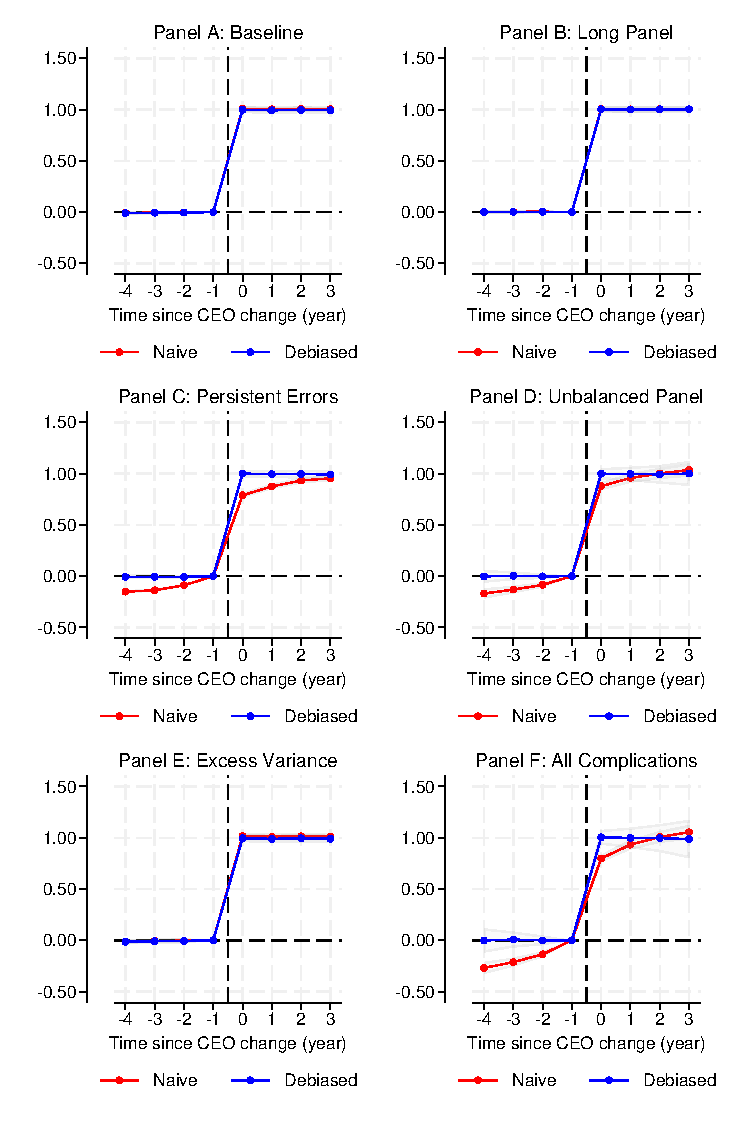
\includegraphics[width=0.8\textwidth]{figure/figuremc.pdf}
\caption{Monte Carlo event studies under six scenarios.} \label{fig:mc}
\vspace{.2cm}

\begin{minipage}{0.9\textwidth}
\footnotesize Notes: Event-time dynamics of variance and covariance in Monte Carlo simulations. Panels A–B: Baseline scenario with i.i.d. shocks ($\rho=0$, $T_1=T_2=5$). Panels C–D: Persistent shocks and unbalanced panel ($\rho=0.9$). Panels E–F: All complications (persistent shocks, unbalanced panels,
excess variance in treated group). Red lines show treated firms, black lines show control (placebo)
firms, blue lines show variance-corrected control. True CEO effect variance $\sigma^2_z=1$. Panels
A, C, E display variance of revenue changes by event time. Panels B, D, F display covariance of
revenue change with CEO effect change. Event time $t=0$ marks CEO transition. In panels A–D, black
and blue lines overlap (no excess variance). In panels E–F, blue line applies excess variance
correction factor $c$ estimated from pre-transition periods.
\end{minipage}
\end{figure}

\begin{figure}[htbp]
\centering
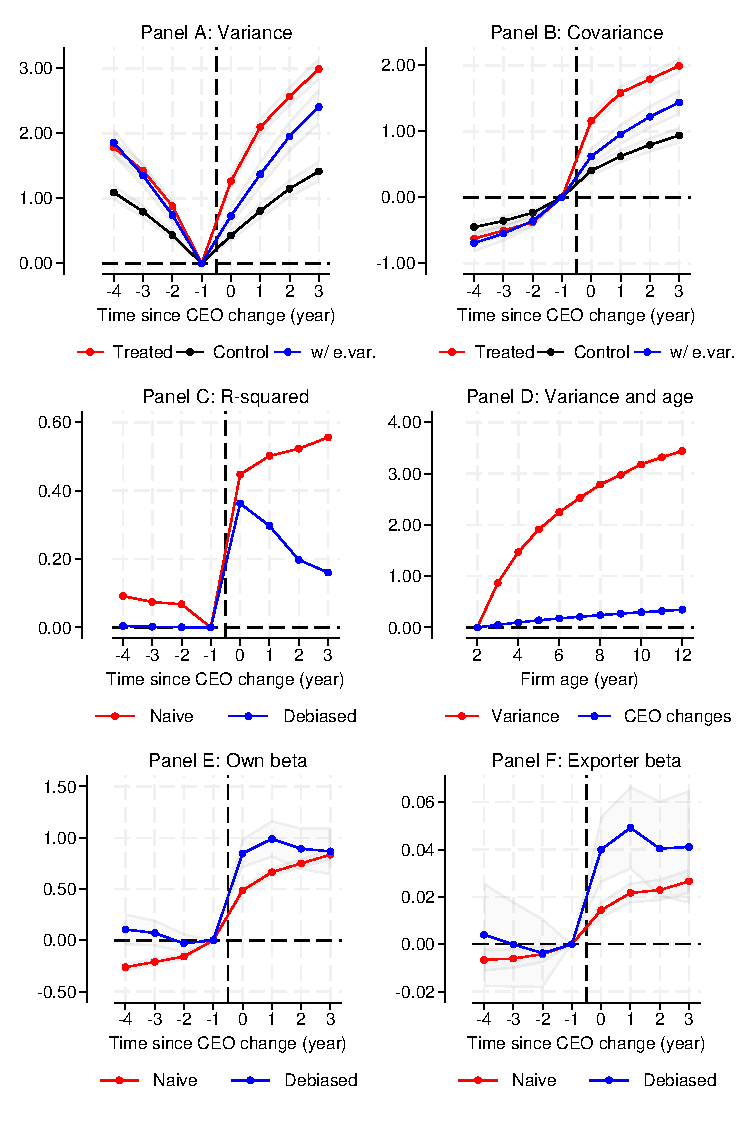
\includegraphics[width=0.9\textwidth]{figure/application.pdf}
\caption{Revenue Dynamics Around CEO Transitions in Hungarian Firms}
\label{fig:application}
\vspace{.2cm}

\begin{minipage}{0.9\textwidth}
\footnotesize
Notes: Event studies of various second moments around CEO transitions. All panels normalize to year $t=-1$ (one year before CEO arrival). Panel A shows the variance of revenue changes from baseline. Panel B plots the covariance of revenue change with the change in CEO fixed effect. Panel C displays the fraction of revenue variance explained by CEO fixed effects (R-squared). Panel D shows the variance of CEO fixed effects by firm age, decomposed into revenue shocks and CEO contributions. Panel E shows regression coefficients from projecting revenue on CEO effects, and Panel F shows the coefficients from regressing exporter status on CEO effect. Red lines show naive OLS estimates; blue lines show placebo-corrected debiased estimates. Shaded regions indicate 95\% confidence intervals. The placebo group consists of matched non-changing firms from the same birth cohort and sector, assigned pseudo CEO transitions at the same calendar year as treated firms. Event window spans $[-4, +3]$ years around CEO arrival.
\end{minipage}
\end{figure}

\begin{table}[t]
\centering
\caption{Monte Carlo parameters by scenario}
\label{tab:mc_params}
\begin{threeparttable}
\begin{tabular}{l*{6}{>{\centering\arraybackslash}p{1.8cm}}}
\toprule
\textbf{Scenario} & \textbf{Baseline} & \textbf{Long Panel} & \textbf{Persistent Errors} & \textbf{Unbalanced Panel} & \textbf{Excess Variance} & \textbf{All Complications} \\
\midrule
\textbf{Parameters} & & & & & & \\
\addlinespace
$N_{\text{treated}}$ & \multicolumn{6}{c}{50,000} \\
$N_{\text{control}}$ & \multicolumn{6}{c}{50,000} \\
$\sigma(\Delta z)$ & \multicolumn{6}{c}{1.00} \\
$\sigma(\epsilon_{\text{control}})$ & \multicolumn{6}{c}{0.71} \\
\addlinespace
 $T_{\max}$ & 5 & 20 & 5 & 5 & 5 & 5 \\
 $\rho$ & 0.00 & 0.00 & 0.90 & 0.90 & 0.00 & 0.90 \\
 $\sigma(\epsilon_{\text{treated}})$ & 0.71 & 0.71 & 0.71 & 0.71 & 1.00 & 1.00 \\
 CEO change & --- & --- & --- & 0.20 & --- & 0.20 \\
 hazard & & & & & & \\
\midrule
\textbf{Estimates} & & & & & & \\
\\ $\sigma(\Delta \hat z)$ (OLS) & $0.104^{}$ & $0.101^{}$ & $0.123^{}$ & $0.118^{}$ & $0.109^{}$ & $0.137^{}$\\ $\sigma(\Delta \hat z)$ (debiased) & $0.100^{}$ & $0.100^{}$ & $0.100^{}$ & $0.100^{}$ & $0.105^{}$ & $0.122^{}$\\ \addlinespace $ R^2$ (OLS) & $0.738^{}$ & $0.686^{}$ & $0.787^{}$ & $0.857^{}$ & $0.584^{}$ & $0.786^{}$\\ $ R^2$ (debiased) & $0.662^{}$ & $0.668^{}$ & $0.593^{}$ & $0.598^{}$ & $0.417^{}$ & $0.267^{}$\\ \addlinespace$\hat \beta_2$ (OLS) & $1.007^{}$ & $1.004^{}$ & $0.933^{***}$ & $1.003^{}$ & $1.015^{}$ & $1.008^{}$\\ $\hat \beta_2$ (debiased) & $0.996^{}$ & $1.002^{}$ & $0.993^{}$ & $0.986^{}$ & $0.892^{***}$ & $0.660^{***}$\\ \addlinespace$\hat \beta_{-2}$ (OLS) & $-0.003^{}$ & $0.004^{}$ & $-0.089^{***}$ & $-0.085^{***}$ & $-0.004^{}$ & $-0.137^{***}$\\ $\hat \beta_{-2}$ (debiased) & $-0.004^{}$ & $0.003^{}$ & $-0.007^{}$ & $-0.001^{}$ & $-0.005^{}$ & $-0.000^{}$\\
\bottomrule
\end{tabular}
\begin{tablenotes}[flushleft]\footnotesize
\item Notes: Every Monte Carlo simulation assumes 50,000 treated firms and 50,000 control firms. The standard deviation of true CEO effect changes is 1.00 and the standard deviation of errors in the control group is 0.71 in all scenarios. The table lists scenario-specific parameters: maximum spell length $T_{\max}$, error autocorrelation $\rho$, error standard deviation in the treated group $\sigma(\epsilon_{\text{treated}})$, and the annual hazard of CEO change in the unbalanced panel scenarios. The \emph{baseline} calibration assumes short balanced spells and i.i.d. errors. Columns (2) to (5) introduce one complication at a time. The \emph{long panel} scenario extends the length of spells. The \emph{persistent errors} scenario adds strong autocorrelation. The \emph{unbalanced panel} scenario introduces firm-specific spell lengths drawn from a geometric distribution with a constant hazard of CEO change. The \emph{excess variance} scenario adds a 50\% increase in error volatility in the treated group relative to the control group. The \emph{all complications} scenario combines unbalanced spells, persistent errors, and excess variance. Parameter values are chosen to represent realistic moments from our application where CEO tenures are often short, revenue shocks are persistent, and treated firms are more volatile than control firms.
\end{tablenotes}
\end{threeparttable}
\end{table}

\end{document}
